\documentclass[12pt,a4paper]{article}

% ============================================================
% Packages
% ============================================================
\usepackage[utf8]{inputenc}
\usepackage[T1]{fontenc}
\usepackage{lmodern}
\usepackage[english]{babel}
\usepackage{csquotes}
\usepackage{amsmath,amssymb}
\usepackage{booktabs}
\usepackage{tabularx}
\usepackage{adjustbox}
\usepackage{graphicx}
\usepackage{xcolor}
\usepackage{hyperref}
\usepackage{cleveref}
\usepackage{float}

% APA citations via biblatex
\usepackage[style=apa,backend=biber,natbib=true]{biblatex}
\addbibresource{references.bib}
\DeclareLanguageMapping{english}{english-apa}

% ============================================================
% Custom commands
% ============================================================
\newcommand{\xscore}{\textit{xScore}}
\newcommand{\xvoa}{\textit{xVOA}}
\newcommand{\gds}{\textit{GDS}}

% Formatting
\emergencystretch=1.5em
\widowpenalty=10000
\clubpenalty=10000

\title{Offense Wins Championships: A Multi-Method Test\\of the Defensive Dominance Hypothesis in the Modern NFL}
\author{Lasse Mecha}
\date{June 2026}

\begin{document}
\maketitle

% ============================================================
% ABSTRACT
% ============================================================
\begin{abstract}
The aphorism ``defense wins championships'' is perhaps the most widely cited empirical claim in professional American football, yet it has received remarkably little rigorous academic testing. We subject this claim to the first systematic, multi-method examination using a machine-learning-derived team quality decomposition. Using the \xscore{} expected-points model and Game Deserved Score (\gds{}) framework \citep{mecha2026xscore-model, mecha2026gds}, we decompose 224 team-seasons (32 teams $\times$ 7 seasons, 2018--2024) into offensive and defensive expected value over average (\xvoa{}) components and classify teams by archetype dominance. Three directional hypotheses operationalizing the defensive claim are tested via five statistical procedures: Spearman rank correlation, Pearson correlation with $R^2$ decomposition, binary logistic regression, OLS regression, and Cohen's $d$ effect size estimation. All three hypotheses are rejected. Offense-dominant teams dramatically outperform defense-dominant teams in playoff advancement (Cohen's $d = 0.672$, 95\% CI $[0.574, 0.787]$), offensive \xvoa{} explains 3.3 times more win-percentage variance than defensive \xvoa{} (46.4\% vs.\ 14.2\%), and all seven Super Bowl champions in the study window were offense-dominant (offense share range: $+0.581$ to $+0.923$). No defense-dominant team won more than one playoff game across 94 playoff team-seasons. Robustness checks -- including opponent-strength controls, field-position mediation analysis, threshold sensitivity, and time-window variation -- confirm that the offensive advantage is structurally stable and not an artifact of schedule strength or measurement choices. We propose a ``competent defense threshold'' framework: offensive excellence drives championship contention while defensive adequacy serves as a necessary but insufficient secondary condition. These findings carry implications for salary-cap allocation strategy in constrained roster-construction environments.
\end{abstract}

\textbf{Keywords:} NFL analytics, defense wins championships, team quality decomposition, expected points, playoff prediction, salary cap allocation

% ============================================================
% 1. INTRODUCTION
% ============================================================
\section{Introduction}
\label{sec:introduction}

The National Football League is the most commercially valuable sports league in the world, with annual revenues exceeding \$22 billion. Each of the league's 32 franchises operates under a hard salary cap -- set at \$301.2 million per team for 2026 \citep{nfl2026cap} -- that imposes a strict zero-sum constraint on roster construction. Unlike the soft-cap systems found in the NBA or the uncapped environments of European football, the NFL's hard cap is strictly enforced: teams that are not cap-compliant by the start of each league year are blocked from signing players and face league-imposed fines \citep{nflcba2020}. While teams can manipulate the timing of cap charges through restructures and void years, these tools merely shift obligations into future seasons rather than eliminating them. The cap does not distinguish between offensive and defensive spending -- it is a single ceiling on total player costs. But precisely because the total is fixed, every allocation decision is implicitly a trade-off: cap space committed to an elite pass-rusher is cap space unavailable for an elite wide receiver. How a franchise divides its finite budget between offense and defense is therefore one of the most consequential strategic choices it faces.

The significance of this constraint becomes apparent when one considers the competitive margins involved. In a 17-game regular season, the difference between making and missing the playoffs is frequently a single victory. The marginal value of roster optimization is enormous, and at a combined annual salary expenditure approaching \$10 billion across all clubs, even a modest misallocation of 5--10\% driven by a faulty heuristic represents cumulative opportunity cost in the hundreds of millions per year. The question of how to allocate between offense and defense admits no neutral answer, and the stakes of getting it wrong are considerable.

For decades, the most pervasive belief surrounding this allocation has been captured in a single phrase: ``offense wins games, defense wins championships.'' The saying is widely attributed to Paul ``Bear'' Bryant, the University of Alabama head coach who won six national championships between 1958 and 1982 \citep{williams2010bearbryant}, though no reliable primary source confirms the attribution. The phrase pervades every level of NFL culture: coaching philosophy (defensive-minded coaches are praised for building ``championship-caliber'' rosters), media narrative (television analysts invoke it each January), and player discourse (players themselves perpetuate it after victories). It articulates a specific and testable empirical claim -- that while offensive quality may drive regular-season success, defensive quality becomes decisive in the postseason. The implied mechanism is intuitive: in playoff games between evenly matched teams, the ability to suppress the opponent's scoring becomes more valuable than the ability to generate one's own, because high-pressure environments compress offensive efficiency while defensive intensity remains sustainable.

Yet the empirical basis for this claim is remarkably thin, and the NFL's competitive landscape has shifted dramatically in recent decades. Beginning with the 2004 ``Ty Law Rule'' restricting defensive contact beyond five yards \citep{nflops2004rules}, and continuing through expanded roughing-the-passer protections and restrictions on defensive physicality \citep{pereira2018roughing}, the league has systematically tilted the environment toward passing offenses. Offensive formations have exploited these changes through the spread revolution, RPO concepts, and pre-snap motion. The result has been a sustained increase in passing efficiency and overall scoring: passer ratings, completion percentages, yards per attempt, and scoring rates have all risen markedly \citep{barnwell2019passingrevolution, nflscoring2023trends}. The 2020s have produced the highest-scoring seasons in NFL history. If the relationship between defensive quality and championship success ever held in a run-dominated, low-scoring era, its persistence in the modern, offense-friendly environment is an open empirical question requiring systematic investigation rather than appeal to tradition.

Despite the claim's financial consequences, rigorous testing has been remarkably scarce. \citet{robst2011defense} published what remains the only direct peer-reviewed examination of the hypothesis in American football. Using data from 1981 through 2009, they employed logistic regression to predict Super Bowl participation and victory from a battery of traditional performance metrics: total offensive yards, total defensive yards allowed, points scored, points allowed, turnover differential, and strength of schedule. Their central finding was that offensive metrics -- particularly points scored and offensive yards -- were substantially stronger predictors of Super Bowl appearance and victory than defensive metrics. They concluded that the ``defense wins championships'' maxim lacks empirical support. However, their independent variables -- total yards and total points -- are aggregate measures that conflate quality with opportunity and context. A team protecting a large lead allows ``garbage time'' yards that inflate defensive statistics without reflecting genuine weakness; an excellent defense on a bad team faces additional possessions because its offense goes three-and-out. Furthermore, no machine learning was employed, no expected-performance baseline was constructed, no game-state conditioning was applied, and no drive-level granularity was available. Their sample predated the modern passing revolution, limiting applicability to the contemporary NFL. No subsequent peer-reviewed study has revisited the hypothesis with modern analytical tools. The grey literature -- blogs, podcasts, social media -- debates the question extensively but relies on selective examples, small-sample anecdotes, or proprietary metrics that cannot be independently verified.

What has been missing is a framework satisfying four properties simultaneously: a calibrated probability baseline (estimating what a league-average team would produce in any situation), an explicit component decomposition (separating offensive, defensive, and special teams contributions on a common scale), full open-source reproducibility (enabling any researcher to replicate or extend the analysis), and pre-specified hypothesis tests (moving beyond anecdote to formal statistical evaluation). The \xscore{} model \citep{mecha2026xscore-model} provides calibrated drive-outcome probabilities from seven situational features, producing a league-average expected-performance baseline. The Game Deserved Score (\gds{}) framework \citep{mecha2026gds} translates these predictions into three additive team quality components -- offensive \xvoa{}, defensive \xvoa{}, and special teams value -- expressed on a common expected-points scale. Together, they provide the measurement infrastructure this paper applies to the championship hypothesis.

This paper tests the following research question: \emph{Is defensive dominance associated with greater playoff success than offensive dominance in the modern NFL?} We operationalize the ``defense wins championships'' claim through three directional hypotheses:

\begin{description}
  \item[H1 (Postseason advancement).] Defense-dominant team-seasons (offense share $< -0.3$) achieve higher mean playoff-win totals than offense-dominant team-seasons (offense share $> +0.3$).
  \item[H2 (Super Bowl over-representation).] Super Bowl winners are disproportionately drawn from defense-dominant team-seasons relative to the base rate of defense dominance among all playoff qualifiers.
  \item[H3 (Correlation asymmetry).] Defensive \xvoa{} per game exhibits a stronger monotonic association with playoff wins among playoff teams than offensive \xvoa{} per game does.
\end{description}

Each hypothesis is stated so that support would be consistent with the defensive narrative. The three are logically independent: H1 concerns mean playoff advancement across the full sample, H2 concerns the extreme tail (one Super Bowl champion per season), and H3 concerns marginal correlations between individual components and outcomes. This independence ensures that any finding is not an artifact of a single operationalization. If all three are supported, the evidence favors the defensive claim. Rejection of any single hypothesis constitutes evidence against it; convergent rejection across all three would provide strong grounds for the opposite conclusion.

This study makes four contributions to the sports analytics literature. First, it provides the first multi-method test of the defensive hypothesis using a calibrated machine-learning decomposition -- extending the crude box-score approach of \citet{robst2011defense} with drive-level measurement, a modern sample, and five converging statistical procedures. Second, it employs pre-specified directional hypotheses tested via five distinct methods to ensure conclusions are robust to methodological choice rather than an artifact of a single test. Third, it introduces the ``competent defense threshold'' as a theoretical framework that moves beyond binary offense-versus-defense framing to articulate a nuanced strategic principle. Fourth, the entire pipeline -- from publicly available data through model training and decomposition to hypothesis testing -- is fully open-source and reproducible \citep{carl2021nflfastr}, enabling any researcher to replicate, extend, or challenge the findings.

% ============================================================
% 2. RELATED WORK
% ============================================================
\section{Related Work}
\label{sec:related-work}

\subsection{The ``Defense Wins Championships'' Debate}
\label{sec:dwc-debate}

The phrase ``defense wins championships'' occupies a peculiar position in sports discourse: it is perhaps the most widely cited empirical claim in professional football, yet it functions simultaneously as folk wisdom, strategic prescription, and empirical hypothesis. Its persuasive power derives partly from its ambiguity -- by remaining vague about the precise mechanism, magnitude, and conditions under which defense ``wins'' championships, the claim resists straightforward falsification while maintaining rhetorical force.

\citet{robst2011defense} published the most direct peer-reviewed examination of the hypothesis. Using data from 1981 through 2009, they employed logistic regression to predict Super Bowl participation and victory from traditional performance metrics: total offensive yards, total defensive yards allowed, points scored, points allowed, turnover differential, and strength of schedule. Their central finding was that offensive metrics -- particularly points scored and offensive yards -- were substantially stronger predictors of Super Bowl appearance and victory than defensive metrics. They concluded that the maxim lacked empirical support. The directional conclusion of the present study is entirely consistent with their finding.

The methodological advance offered by the \gds{} framework over their approach is considerable, however. Their analysis relied on traditional box-score statistics that conflate quality with volume and fail to account for game context. A team protecting a large lead frequently allows yards and points in garbage time that inflate its defensive statistics without reflecting genuine weakness; a team trailing throws aggressively in desperation, accumulating passing yards against prevent defenses. No machine learning was employed, no game-state conditioning was applied, and no drive-level granularity was available. The \xscore{} model addresses these limitations by conditioning drive-outcome probabilities on field position, down, distance, score differential, and time remaining, providing a calibrated baseline that accounts for game state \citep{mecha2026xscore-model}. This context-sensitivity represents a substantial refinement over raw box-score approaches.

No subsequent peer-reviewed study has directly revisited the hypothesis with modern analytical tools in the 15 years since Robst et al.'s publication. Football Outsiders' DVOA provides an offense/defense decomposition and implicitly supports offensive primacy in its published rankings, but its proprietary, non-reproducible methodology prevents independent verification -- claims rest on authority rather than transparency \citep{schatz2005dvoa}. The present study fills this gap with a fully specified, publicly verifiable framework.

\subsection{Postseason Prediction and Randomness}
\label{sec:prediction-randomness}

Any investigation of championship predictors in the NFL must contend with the dominant role of randomness in single-elimination playoffs. A team plays at most four postseason games en route to a Super Bowl victory, meaning that a single turnover, injury, or officiating decision can end a season regardless of overall quality \citep{lopez2018randomness}. This high variance creates a fundamental tension: if randomness dominates single-game outcomes, the relationship between any quality dimension and championship success will necessarily be weak, and large samples are required to detect genuine effects. Multi-season aggregation is essential for disentangling signal from noise.

\citet{lock2014randomforests} demonstrated that random forests predicting NFL game outcomes found offensive variables -- particularly passing efficiency metrics -- consistently more predictive of wins than defensive variables. Their machine-learning approach, operating at the game level with different features and modeling strategy, reached the same directional conclusion as the present drive-level analysis. This convergence across methodological traditions suggests the finding is robust to analytic framework rather than an artifact of any particular measurement approach.

The present study addresses the randomness concern through a 224 team-season sample spanning seven complete NFL cycles (2018--2024), five statistical methods with different assumptions and sensitivities, and a convergence requirement: conclusions rest on consistency across all procedures rather than any single $p$-value crossing a threshold.

\subsection{Resource Allocation Under Salary Cap Constraints}
\label{sec:resource-allocation-lit}

The NFL's hard salary cap creates a zero-sum dynamic that distinguishes it from most other professional sports leagues. In Major League Baseball, teams with larger revenues can simply outspend smaller-market competitors \citep{lewis2003moneyball}. The NFL's hard cap eliminates this avenue: every team has precisely the same budget, and the only variable is how that budget is allocated. This zero-sum property is what makes the offense-defense allocation question consequential -- if one strategy is superior, teams pursuing the inferior strategy face a systematic disadvantage that cannot be compensated through increased spending. The operations research literature on constrained optimization under uncertainty provides the theoretical framework: optimal allocation depends on the marginal return per unit of investment in each asset class.

\citet{mulholland2019optimizing} provided the most direct treatment of the allocation optimization problem, developing a model for how NFL teams should distribute salary cap funds across positions to maximize performance. Their analysis quantified the marginal win-value of spending at each position group, finding substantial heterogeneity in returns. Quarterback spending emerged as the single most efficient allocation, consistent with the broader finding that offensive quality drives winning. The gap between current league-average allocation and theoretically optimal allocation was substantial -- teams collectively leave wins on the table through suboptimal positional spending, providing economic grounding for the strategic implications of the present study.

\citet{massey2013loserscurse} demonstrated that NFL teams systematically overvalue early draft picks relative to the surplus production those selections generate. Their ``Loser's Curse'' finding implies a market inefficiency in talent acquisition that compounds the allocation problem. If the ``defense wins championships'' heuristic drives teams to deploy premium draft capital on defensive players (edge rushers, cornerbacks, defensive tackles), and if offensive investment actually delivers superior championship returns, the resulting misallocation is doubly inefficient: teams invest in the wrong side of the ball using the most overpriced acquisition mechanism available. The rational strategy, if the present findings reflect causal mechanisms, would be to acquire offensive talent through the draft (where rookie contracts provide below-market cost) and fill defensive needs through free agency. The team that correctly identifies offensive quality as the stronger championship predictor can exploit the systematic mispricing that the defensive heuristic creates.

\subsection{Contribution of This Study}
\label{sec:contribution}

Four contributions distinguish this paper from prior work. First, the \gds{} framework provides the first fully open-source, reproducible team quality metric with an explicit three-component decomposition used for formal hypothesis testing -- addressing the reproducibility gap left by proprietary systems like DVOA. Second, drive-level probability modeling rather than play-level EPA respects the natural possession structure of American football, avoids the well-documented issues with play-level aggregation (within-drive non-independence, game-script contamination, outcome conflation), and provides the calibrated baseline that downstream quality measurement requires \citep{mecha2026xscore-model}. Third, this paper provides the first systematic, multi-method test of the defensive hypothesis using five statistical procedures applied to 224 team-seasons with pre-specified directional hypotheses -- providing considerably stronger evidence than any single prior study. Fourth, the ``competent defense threshold'' concept formalizes a nuanced position that moves beyond the binary ``offense versus defense'' debate, articulating a strategic principle: elite teams invest in defensive competence to avoid catastrophic vulnerability while allocating marginal resources toward offensive excellence, where the championship return on investment is substantially higher.

% ============================================================
% 3. DATA AND METHODS
% ============================================================
\section{Data and Methods}
\label{sec:methods}

\subsection{Measurement Framework}
\label{sec:measurement}

The probability baseline is provided by \xscore{} \citep{mecha2026xscore-model}, a calibrated multinomial XGBoost model that predicts four mutually exclusive drive outcomes -- touchdown, field goal, turnover, punt/other -- from seven situational features describing the game state at the drive's start: down, yards to go, field position (yardline), score differential, time remaining in half, a goal-to-go indicator, and a red zone indicator. Team identity is deliberately excluded from the feature set, producing a league-average expected-performance baseline independent of who is playing -- deviations from this baseline therefore measure team quality rather than circular self-prediction. The model is trained on 241,195 plays from seven NFL seasons (2018--2024) and achieves a multiclass Brier score of 0.1562 on a held-out 2025 test set (Brier Skill Score 15.3\% over a naive marginal-frequency baseline), with a mean Expected Calibration Error of 0.010 confirming that predicted probabilities closely match observed outcome frequencies across the full probability range. Per-class isotonic calibration ensures this property holds for each outcome category individually. The four-class probability vector converts to a single expected-points figure via a weighted formula that assigns 7 points to touchdowns, 3 to field goals, 0 to punts, and a field-position-dependent penalty to turnovers. Calibration is essential because downstream \xvoa{} calculations treat predicted probabilities as genuine expected values from which deviations carry quantitative meaning; systematic miscalibration would propagate into biased team quality estimates.

The Game Deserved Score (\gds{}) framework \citep{mecha2026gds} translates \xscore{} predictions into a three-component team quality metric. For each drive, offensive \xvoa{} (expected Value Over Average) equals the actual points scored by the offense minus the \xscore{}-predicted expected points from that starting state. A drive that produces a touchdown when the model predicted 3.2 expected points generates $+3.8$ offensive \xvoa{}; a drive that punts when the model predicted 2.1 expected points generates $-2.1$ offensive \xvoa{}. Positive values indicate the offense exceeded expectations; negative values indicate underperformance relative to what a league-average team would produce from the same situation. Defensive \xvoa{} is constructed analogously from the opponent's offensive drives: when the opposing offense scores less than expected, the defense receives positive \xvoa{}, reflecting its contribution to suppressing opponent scoring. A special teams component (ST\_Value) captures field-position deviations from transition-type baselines. The three components sum to a total \gds{} for each game and can be averaged across games to produce season-level team quality estimates.

At the season level, mean \gds{}/game correlates $r = 0.858$ with win percentage ($R^2 = 73.6\%$, $n = 224$ team-seasons), confirming that the framework captures genuine team quality at a level substantially exceeding point differential or traditional metrics. The team with higher \gds{} wins 86.1\% of regular-season games. Full derivation, construction, and validation are reported in the companion paper \citep{mecha2026gds}; the reader need only accept that \xscore{} produces calibrated drive-outcome probabilities and \gds{} decomposes these into offensive, defensive, and special teams quality signals.

\subsection{Sample and Variables}
\label{sec:sample}

The analysis operates on 224 team-seasons (32 teams across 7 seasons, 2018--2024). The 2018 lower bound reflects the structural break in scoring distributions created by rule changes; the 2024 upper bound is the most recent completed season. The playoff subsample comprises 94 team-seasons -- roughly 13--14 per season, accounting for the bracket expansion from 12 to 14 teams in 2020. The Super Bowl winner subsample contains exactly 7 observations, one per season. All independent variables are computed from regular-season games only to ensure temporal separation from dependent variables measuring postseason outcomes.

\Cref{tab:ivs} defines the four independent variables used in the analysis.

\begin{table}[htbp]
  \centering
  \caption{Independent variables in the archetype analysis. All variables are
           computed at the team-season level using regular-season games only.
           Per-game averages remove the effect of schedule length variation.}
  \label{tab:ivs}
  \begin{tabularx}{\textwidth}{llX}
    \toprule
    \textbf{Variable} & \textbf{Type} & \textbf{Definition} \\
    \midrule
    \texttt{offense\_share}
      & Continuous $[-1, +1]$
      & Proportion of total absolute \xvoa{} attributable to the offense
        (see \Cref{eq:offense-share}). Positive values indicate
        offense-dominant teams; negative values indicate defense-dominant teams. \\[6pt]
    \texttt{gds\_per\_game}
      & Continuous
      & Mean \gds{} per regular-season game. Measures overall team quality
        in expected-point units, independent of offensive/defensive split. \\[6pt]
    \texttt{off\_xvoa\_per\_game}
      & Continuous
      & Mean offensive \xvoa{} per regular-season game. Direct measure of
        offensive output above or below situational expectation. \\[6pt]
    \texttt{def\_xvoa\_per\_game}
      & Continuous
      & Mean defensive \xvoa{} per regular-season game. Direct measure of
        defensive suppression above or below expectation.
        Positive values indicate above-average defensive performance. \\
    \bottomrule
  \end{tabularx}
\end{table}

The key analytical variable is \texttt{offense\_share}, which isolates the \emph{balance} between offensive and defensive contribution independently of overall team quality:

\begin{equation}
  \label{eq:offense-share}
  \texttt{offense\_share} =
  \frac{\texttt{off\_xvoa\_per\_game}}
       {|\texttt{off\_xvoa\_per\_game}| + |\texttt{def\_xvoa\_per\_game}| + \varepsilon},
\end{equation}

where $\varepsilon = 0.01$ is a small regularization constant preventing division by zero for teams with negligible \xvoa{} in both channels. The denominator is the sum of absolute magnitudes, so the ratio measures the fraction of the team's total absolute performance attributable to offense. The $\varepsilon$ term does not materially affect results for any team with non-trivial \xvoa{}, since realistic per-game magnitudes are on the order of 1--12 expected-point units. The resulting variable ranges from $-1$ to $+1$ by construction; in practice most team-seasons fall in $[-0.6, +0.6]$. The defense-dominant threshold is set at offense share $< -0.3$; the offense-dominant threshold at $> +0.3$. Sensitivity analysis tests alternative thresholds from $\pm 0.20$ to $\pm 0.40$.

\Cref{tab:dvs} defines the three dependent variables.

\begin{table}[htbp]
  \centering
  \caption{Dependent variables. Playoff wins counts actual games won in the
           postseason; bye weeks are not treated as wins because no game was played.}
  \label{tab:dvs}
  \begin{tabularx}{\textwidth}{llX}
    \toprule
    \textbf{Variable} & \textbf{Type} & \textbf{Description} \\
    \midrule
    \texttt{win\_pct}
      & Continuous $[0, 1]$
      & Regular-season win fraction. Used to assess whether \xvoa{} components
        predict season-level success. \\[6pt]
    \texttt{playoff\_wins}
      & Ordinal $\{0, 1, 2, 3, 4\}$
      & Number of postseason games won. A value of 0 indicates either missing
        the playoffs or a first-round exit. A Super Bowl winner receives 3 (with
        first-round bye) or 4 (playing Wild Card round). \\[6pt]
    \texttt{won\_super\_bowl}
      & Binary $\{0, 1\}$
      & Indicator for Super Bowl victory. \\
    \bottomrule
  \end{tabularx}
\end{table}

\subsection{Hypotheses}
\label{sec:hypotheses}

The three hypotheses stated in \Cref{sec:introduction} are designed to decompose the ``defense wins championships'' claim into three independent, falsifiable components. H1 tests whether defensive dominance predicts deeper playoff runs (a population-level mean comparison). H2 tests whether the extreme tail -- Super Bowl champions specifically -- favors defense-dominant teams. H3 tests whether the marginal correlation between defensive quality and outcomes exceeds that between offensive quality and outcomes. The logical independence of these tests ensures that convergent rejection provides stronger inferential warrant than any single test could deliver.

\subsection{Statistical Procedures}
\label{sec:procedures}

Five statistical procedures are employed, each motivated by the measurement level and distributional properties of the variables involved. The procedures are designed to converge or diverge as a coherent body of evidence; the inferential conclusion rests on consistency and direction across all five, not on any single $p$-value.

\paragraph{Spearman rank correlation.} The primary test of H1 and H3 computes the Spearman rank correlation between \texttt{offense\_share} and \texttt{playoff\_wins} across all 94 playoff team-seasons. The Spearman coefficient is appropriate because \texttt{playoff\_wins} is ordinal with a bounded range of 0--4 (treating it as interval-scaled would impose an equal-spacing assumption that may not hold), and the potentially non-linear monotonic relationship between team balance and playoff success is better captured by a rank-based measure. A positive coefficient indicates that offensive dominance predicts playoff advancement; a negative coefficient would support the defensive hypothesis. A 95\% bootstrap confidence interval is reported.

\paragraph{Pearson correlation with $R^2$ decomposition.} Pearson product-moment correlations are computed between offensive \xvoa{}/game and win percentage, and between defensive \xvoa{}/game and win percentage, across all 224 team-seasons. The use of Pearson is appropriate here because win percentage is a continuous proportion that is approximately normally distributed at the team-season level, and the linear relationship between per-game \xvoa{} and season win rate is theoretically motivated by the additive structure of the \gds{} framework. The squared correlations ($R^2$) provide a direct comparison of variance explained: if H3 were supported, the defensive $R^2$ should exceed the offensive $R^2$.

\paragraph{Binary logistic regression.} To test H2, a binary logistic regression models Super Bowl victory as a function of offensive and defensive \xvoa{}/game across all 224 team-seasons:
\begin{equation}
  \label{eq:logistic}
  \log \frac{P(\texttt{won\_SB} = 1)}{P(\texttt{won\_SB} = 0)}
  = \beta_0
    + \beta_1 \cdot \texttt{off\_xvoa/g}
    + \beta_2 \cdot \texttt{def\_xvoa/g}.
\end{equation}
A finding of $|\hat{\beta}_2| > |\hat{\beta}_1|$ would be consistent with H2. Standard errors, Wald $z$-statistics, and $p$-values are reported. With only 7 Super Bowl winners and 2 predictors, the events-per-variable (EPV) ratio is 3.5, well below the recommended minimum of 10 \citep{hosmer2013logistic, peduzzi1996simulation}. The model is therefore interpreted as directional and exploratory; coefficient magnitudes and signs are examined but $p$-values are treated as approximate.

\paragraph{OLS regression.} An OLS regression of \texttt{playoff\_wins} on \texttt{off\_xvoa\_per\_game} and \texttt{def\_xvoa\_per\_game} across all 224 team-seasons:
\begin{equation}
  \label{eq:ols}
  \texttt{playoff\_wins}_i
  = \alpha
    + \beta_1 \cdot \texttt{off\_xvoa/g}_i
    + \beta_2 \cdot \texttt{def\_xvoa/g}_i
    + \varepsilon_i.
\end{equation}
Although \texttt{playoff\_wins} is technically ordinal, OLS on ordinal outcomes with a small number of categories is widely used in applied social-science research and provides interpretable coefficient estimates \citep{long1997regression}. Because the outcome is zero-inflated (approximately 58\% of team-seasons have zero playoff wins), residuals are heteroscedastic; all reported standard errors use HC3 estimates. The Spearman correlations serve as a non-parametric robustness check that does not impose linearity or equal-interval assumptions.

\paragraph{Cohen's $d$ effect size.} The standardized mean difference in \texttt{playoff\_wins} between offense-dominant (share $> +0.3$, $n = 143$) and defense-dominant (share $< -0.3$, $n = 29$) team-seasons across all 224 observations:
\begin{equation}
  \label{eq:cohens-d}
  d = \frac{\bar{x}_{\mathrm{off}} - \bar{x}_{\mathrm{def}}}{s_p},
  \qquad
  s_p = \sqrt{\frac{(n_{\mathrm{def}} - 1)\,s_{\mathrm{def}}^2
                    + (n_{\mathrm{off}} - 1)\,s_{\mathrm{off}}^2}
                   {n_{\mathrm{def}} + n_{\mathrm{off}} - 2}}.
\end{equation}
Non-playoff team-seasons receive \texttt{playoff\_wins} $= 0$, so the effect size captures both the selection effect (making the playoffs) and the advancement effect (winning once there). Conventional thresholds \citep{cohen1988statisticalpower}: $|d| < 0.2$ is negligible, $|d| \approx 0.2$ is small, $|d| \approx 0.5$ is medium, $|d| \approx 0.8$ is large. A positive $d$ indicates offense-dominant teams win more. A 95\% bootstrap confidence interval is reported.

Additionally, a \textbf{quartile analysis} partitions all 224 team-seasons into four equal groups (56 per quartile) by \texttt{offense\_share} as a non-parametric complement. Q1 contains the most defense-dominant teams; Q4 the most offense-dominant. For each quartile, the analysis reports playoff appearance rate, mean playoff wins, conference championship rate, and Super Bowl win count. If the defensive narrative is correct, outcomes should improve from Q4 to Q1.

\paragraph{Multiple-testing considerations.} No family-wise error rate correction (e.g., Holm--Bonferroni) is applied. The five procedures test the same substantive hypothesis from different angles rather than testing independent hypotheses; the inferential conclusion rests on directional convergence across all five methods rather than on any single $p$-value crossing a significance threshold. This convergence-based approach is more conservative in practice than correction-based approaches because it requires \emph{all} tests to agree rather than any single corrected test to pass.

\subsection{Robustness Design}
\label{sec:robustness-design}

Six robustness checks address potential threats to the validity of the primary findings.

\emph{Opponent-strength control.} The OLS model is re-estimated including a leave-one-out opponent-quality variable (\texttt{opp\_avg\_gds}): for each team-season, the mean \gds{}/game of all opponents faced during the regular season, excluding the focal team's own contribution. The leave-one-out construction prevents the mechanical correlation that would arise if a team's own quality inflated its opponents' apparent strength. If the offensive advantage is an artifact of schedule imbalance -- offense-dominant teams facing weaker schedules -- then including this covariate should attenuate or eliminate the offensive coefficient.

\emph{Field-position mediation.} A plausible alternative explanation is that defensive quality generates favorable starting field position, which inflates offensive \xvoa{}. A mediation analysis \citep{baron1986moderator} quantifies the proportion of the offensive \xvoa{}-to-wins association attributable to defense-generated starting position. The total correlation is compared to the partial correlation controlling for average starting field position advantage.

\emph{Threshold sensitivity.} The defense-dominant classification threshold ($\pm 0.3$) is varied from $\pm 0.20$ to $\pm 0.40$ in increments of 0.05. Mean playoff wins for defense-dominant teams are reported at each threshold to confirm that the null result is not an artifact of the specific boundary chosen.

\emph{Time-window variation.} The offensive-to-defensive $R^2$ ratio is computed across five overlapping time windows (2018--2024, 2018--2022, 2019--2024, 2020--2024, 2018--2021) to confirm the result is not driven by a single anomalous season.

\emph{Single-team exclusion.} Kansas City 2023 -- the lowest offense share among Super Bowl champions ($+0.581$) and the most frequently cited counter-example -- is excluded from all primary analyses to verify conclusions are not dependent on any single observation.

\emph{Era comparison.} The sample is split at 2018--2020 versus 2021--2024, with Spearman and Pearson correlations computed per era. This comparison is explicitly exploratory -- per-era subsamples (38 and 56 playoff team-seasons respectively) are insufficient for formal inference about era differences, and the comparison is intended to assess directional consistency rather than quantify temporal trends.

% ============================================================
% 4. RESULTS
% ============================================================
\section{Results}
\label{sec:results}

\subsection{Descriptive Patterns}
\label{sec:descriptive}

\subsubsection{Offense Share Quartiles}

\Cref{tab:quartile} partitions all 224 team-seasons into four equal groups by \texttt{offense\_share}. Quartile~1 (Q1) contains the 56 most defense-dominant team-seasons (most negative offense share); Quartile~4 (Q4) contains the 56 most offense-dominant.

\begin{table}[htbp]
  \centering
  \caption{Postseason outcomes by \texttt{offense\_share} quartile ($N = 224$
           team-seasons, 2018--2024; 56 per quartile). Avg~PW includes
           non-qualifiers (playoff wins $= 0$). Conf+ is conference
           championship or better.}
  \label{tab:quartile}
  \begin{adjustbox}{max width=\textwidth}
  \begin{tabular}{lcrrrrrr}
    \toprule
    \textbf{Quartile} & \textbf{N}
      & \textbf{Avg Share} & \textbf{Playoff\%}
      & \textbf{Avg PW} & \textbf{Conf+\%} & \textbf{SB Win\%} \\
    \midrule
    Q1 (Defense) & 56 & $-0.373$ & 10.7           & 0.02 & \phantom{0}0.0 & 0.0 \\
    Q2           & 56 & $+0.291$ & 14.3           & 0.05 & \phantom{0}0.0 & 0.0 \\
    Q3           & 56 & $+0.569$ & 55.4           & 0.46 & 12.5           & 1.8 \\
    Q4 (Offense) & 56 & $+0.815$ & 87.5           & 1.02 & 28.6           & 10.7 \\
    \bottomrule
  \end{tabular}
  \end{adjustbox}
\end{table}

\begin{figure}[htbp]
  \centering
  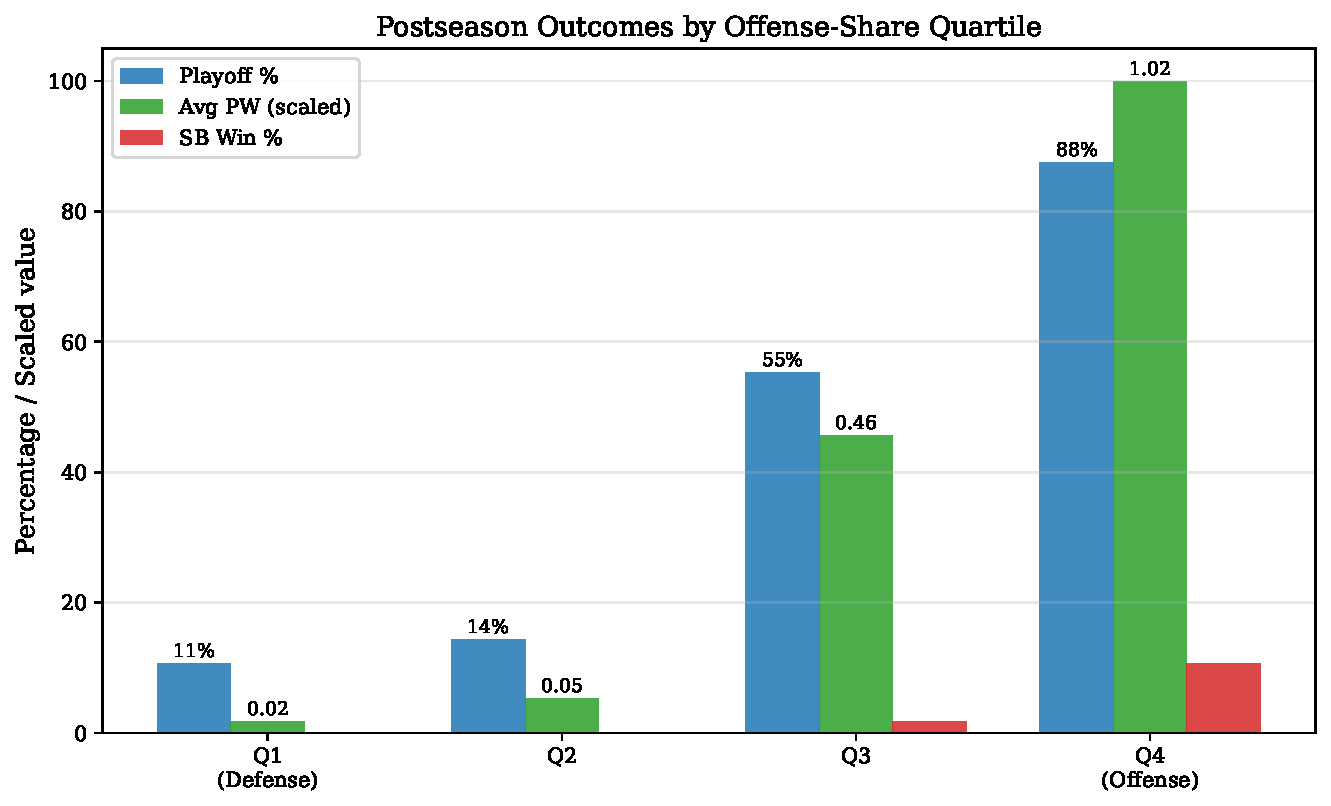
\includegraphics[width=0.85\textwidth]{../../thesis/figures/fig4_quartile_bars.pdf}
  \caption{Postseason outcomes by offense-share quartile. The monotonic
           gradient from Q1 (defense-dominant) to Q4 (offense-dominant) is
           visible across all three metrics: playoff qualification,
           average playoff wins, and Super Bowl victories.}
  \label{fig:quartile-bars}
\end{figure}

The data reveal a monotonic gradient that runs in precisely the opposite direction to the ``defense wins championships'' prediction. Playoff appearance rates increase sharply and continuously from Q1 to Q4: 10.7\% of the most defense-dominant teams made the playoffs, compared to 87.5\% of the most offense-dominant -- an eight-fold difference. Mean playoff wins follow the same gradient: 0.02 in Q1 to 1.02 in Q4, representing a 50-fold difference in expected postseason advancement. The gradient is not merely linear but accelerating: the Q3--Q4 gap (0.46 to 1.02) is larger in absolute terms than the Q1--Q2 gap (0.02 to 0.05), suggesting convexity in the relationship between offensive dominance and playoff advancement.

The conference championship rate provides the starkest illustration of the asymmetry. Not a single team-season in Q1 or Q2 -- collectively the 112 most defense-dominant team-seasons in the dataset -- reached a conference championship game. The first non-zero conference championship rate appears only in Q3 at 12.5\%, and Q4 registers 28.6\%. All seven Super Bowl victories fall in Q3 or Q4; none is attributable to a team in the two most defense-dominant quartiles. The complete absence of deep postseason runs in the bottom half of the offense-share distribution is notable given the large combined sample size of 112 team-seasons.

\subsubsection{Super Bowl Participants}

\Cref{tab:sb-participants} lists all team-seasons that won three or more playoff games during the study window -- comprising all seven Super Bowl winners and the 2021 Cincinnati Bengals (who reached the Super Bowl as a non-bye team with three playoff wins before losing).

\begin{table}[htbp]
  \centering
  \caption{Teams with $\geq 3$ playoff wins, 2018--2024 (all Super Bowl
           winners plus the 2021 runner-up). Off/G and Def/G are mean
           per-game \xvoa{} in expected-point units. Share is
           \texttt{offense\_share}. PW is playoff wins.}
  \label{tab:sb-participants}
  \begin{adjustbox}{max width=\textwidth}
  \begin{tabular}{llrrrrl}
    \toprule
    \textbf{Season} & \textbf{Team}
      & \textbf{Off/G} & \textbf{Def/G}
      & \textbf{Share} & \textbf{PW} & \textbf{SB} \\
    \midrule
    2018 & NE  & $+5.365$ & $-1.177$ & $+0.819$ & 3 & Win \\
    2019 & KC  & $+8.033$ & $-1.982$ & $+0.801$ & 3 & Win \\
    2020 & TB  & $+10.000$ & $-2.719$ & $+0.786$ & 4 & Win \\
    2021 & CIN & $+6.643$ & $-1.436$ & $+0.821$ & 3 &  -- \\
    2021 & LA  & $+8.524$ & $-2.362$ & $+0.782$ & 4 & Win \\
    2022 & KC  & $+10.501$ & $-3.826$ & $+0.732$ & 3 & Win \\
    2023 & KC  & $+2.641$ & $+1.896$ & $+0.581$ & 4 & Win \\
    2024 & PHI & $+7.740$ & $+0.639$ & $+0.923$ & 4 & Win \\
    \bottomrule
  \end{tabular}
  \end{adjustbox}
\end{table}

Several structural observations emerge from this table. Every Super Bowl winner is unambiguously offense-dominant, with offense shares ranging from $+0.581$ (Kansas City 2023) to $+0.923$ (Philadelphia 2024). No defense-dominant team-season reached the Super Bowl during the study window.

Five of the seven champions recorded \emph{negative} defensive \xvoa{}/game, meaning their defenses performed below league-average expectations at the drive level. This counterintuitive finding reinforces the central result: championship teams succeed through offensive surplus, not defensive excellence. Kansas City's 2022 championship is particularly illustrative: their defensive \xvoa{} was $-3.826$/game -- substantially below average -- yet they won the Super Bowl carried entirely by an elite offense ($+10.501$/game). A team can win a championship with a defense performing well below average, provided the offensive surplus is sufficiently dominant.

Kansas City 2023 represents the lowest offense share among champions ($+0.581$), with the smallest offensive \xvoa{} in the group ($+2.641$/game). Unlike their 2022 title, the 2023 team benefited from a positive defensive contribution ($+1.896$/game). This season is often characterized in popular discourse as a ``defense-led'' championship. However, the \gds{} framework reveals that offensive value still exceeded defensive value in absolute terms -- the team was offense-dominant, albeit less dramatically than other champions. The popular narrative that Kansas City's 2023 title validates ``defense wins championships'' is not supported by the expected-point decomposition: it is the \emph{least} offense-dominant champion, not a defense-dominant one.

Philadelphia 2024 achieved the highest offense share among champions ($+0.923$), with a strong offensive \xvoa{} ($+7.740$/game) complemented by modest positive defense ($+0.639$/game). Their profile demonstrates that championship teams need not have elite defense if offensive production is sufficiently dominant.

The empirical headline is stated directly: \textbf{no net-defense team (offense share $< 0$) won more than one playoff game across seven seasons and 94 playoff team-seasons.} Among all 94 playoff team-seasons, only six had negative offense share values. The sole team among them to win any playoff game was Houston 2024 (offense share $= -0.069$, one playoff win). At the stricter defense-dominant threshold of $< -0.3$ used for formal hypothesis testing, zero of 29 such team-seasons won any playoff games whatsoever.

\begin{figure}[htbp]
  \centering
  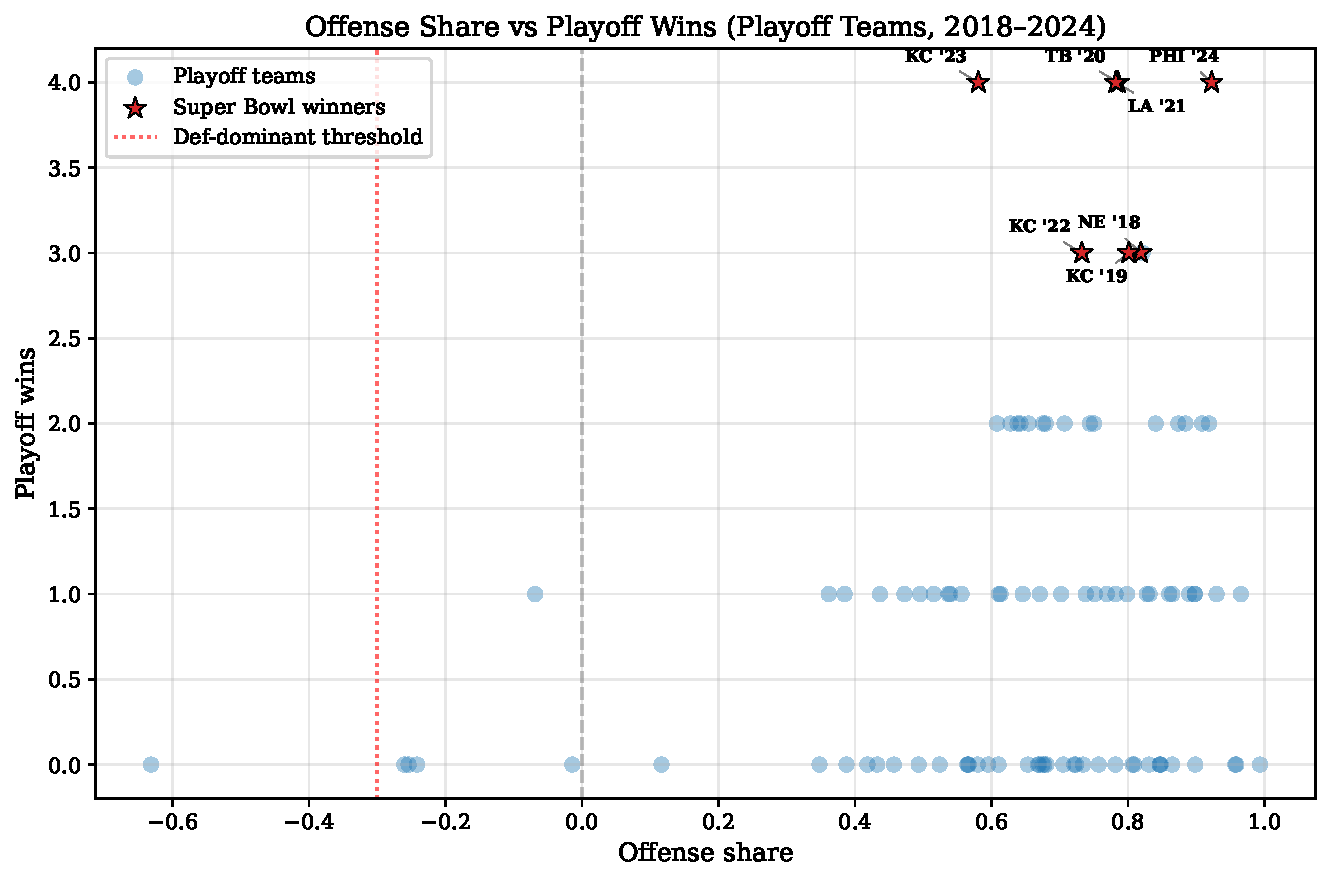
\includegraphics[width=0.85\textwidth]{../../thesis/figures/fig7_offense_share_pw.pdf}
  \caption{Offense share vs.\ playoff wins for all playoff team-seasons
           (2018--2024). Super Bowl winners (annotated) cluster in the
           offense-dominant region. No team below the defense-dominant
           threshold ($< -0.3$) won any playoff games.}
  \label{fig:offense-share-pw}
\end{figure}

\subsection{Hypothesis Tests}
\label{sec:hypothesis-tests}

\subsubsection{Spearman Rank Correlation}

The Spearman rank correlation between \texttt{offense\_share} and \texttt{playoff\_wins} across all 94 playoff team-seasons:
\[
  \rho = 0.246, \quad p = 0.0167, \quad n = 94, \quad \text{95\% bootstrap CI } [0.060,\; 0.423].
\]
The positive sign confirms that higher offense share is associated with more playoff wins: teams whose \gds{} was driven proportionally more by offense won more postseason games on average. The correlation is statistically significant at $\alpha = 0.05$, providing evidence against the null hypothesis of no association. The magnitude ($\rho = 0.246$) is a small-to-medium effect reflecting the inherent noisiness of single-elimination postseason samples. Crucially, this coefficient directly contradicts the directional prediction of H3 -- if the defensive hypothesis were correct, the coefficient should be negative (defensive dominance predicting more wins). The positive sign establishes that offensive dominance, not defensive dominance, predicts playoff advancement.

\subsubsection{Pearson Correlations and $R^2$ Decomposition}

The season-level Pearson correlations between each \xvoa{} component and win percentage across all 224 team-seasons:
\begin{align*}
  r(\text{Off\_xVOA/g},\ \text{Win\%}) &= 0.681,\quad p < 0.000001, \\
  &\quad \text{95\% CI } [0.608,\; 0.743],\quad R^2 = 46.4\%, \\[4pt]
  r(\text{Def\_xVOA/g},\ \text{Win\%}) &= 0.376,\quad p < 0.000001, \\
  &\quad \text{95\% CI } [0.260,\; 0.483],\quad R^2 = 14.2\%.
\end{align*}
Both correlations are highly significant, confirming that each component independently predicts season-level success. However, the magnitudes diverge substantially: offensive \xvoa{} explains $R^2 = 46.4\%$ of the variance in win percentage, while defensive \xvoa{} explains only $R^2 = 14.2\%$ -- a ratio of approximately $3.3 : 1$ in favor of offense. If one were forced to evaluate a team's competitive quality using only one side of the ball, offense would provide more than three times as much information as defense.

This ratio runs in the opposite direction to H3. For H3 to be supported, the defensive coefficient would need to exceed the offensive coefficient; instead, offense dominates by a factor of 3.3. The finding is consistent with the broader NFL analytics literature identifying passing efficiency and drive conversion as primary determinants of team outcomes \citep{yurko2019nflwar}, and extends that literature by replicating the result in expected-point units with a calibrated probability baseline.

\subsubsection{Cohen's $d$ Effect Size}

Cohen's $d$ is computed as the standardized mean difference in playoff wins between offense-dominant ($n = 143$) and defense-dominant ($n = 29$) team-seasons across all 224 observations:
\begin{align*}
  \bar{x}_{\mathrm{off}} &= 0.601 \text{ playoff wins}, \quad n_{\mathrm{off}} = 143, \\
  \bar{x}_{\mathrm{def}} &= 0.000 \text{ playoff wins}, \quad n_{\mathrm{def}} = 29, \\
  d &= 0.672, \quad \text{95\% bootstrap CI } [0.574,\; 0.787].
\end{align*}
The positive $d$ indicates offense-dominant teams win more playoff games, directly contradicting H1. The magnitude is medium-to-large by conventional benchmarks \citep{cohen1988statisticalpower}, and the confidence interval excludes zero by a wide margin. The practical interpretation is the most striking finding of the entire analysis: not a single defense-dominant team-season in the sample won any playoff games whatsoever. Of the 29 defense-dominant team-seasons (offense share $< -0.3$), only one (3.4\%) even qualified for the playoffs, and it was eliminated in the first round. Offense-dominant teams, by contrast, made the playoffs at a 60.8\% rate and averaged 0.60 wins per season -- a difference that operates through both the selection channel (making the playoffs) and the advancement channel (winning once there).

The defense-dominant group is smaller ($n = 29$) than the offense-dominant group ($n = 143$), reflecting the empirical reality that defense-dominant profiles are rarer among competitive teams. The bootstrap confidence interval accounts for this asymmetry, and the lower bound of 0.574 confirms robustness to sampling variability.

\subsubsection{Logistic Regression}

\Cref{tab:logistic} reports the binary logistic regression predicting Super Bowl victory.

\begin{table}[htbp]
  \centering
  \caption{Binary logistic regression predicting Super Bowl victory
           ($N = 224$ team-seasons, 7 winners). Coefficients are
           log-odds. $p$-values are two-tailed Wald tests.}
  \label{tab:logistic}
  \begin{tabular}{lrrrr}
    \toprule
    \textbf{Predictor} & \textbf{Coef.}
      & \textbf{SE}
      & \textbf{$p$} \\
    \midrule
    Offensive \xvoa{}/game & $0.368$ & $0.126$ & $0.0034$ \\
    Defensive \xvoa{}/game & $0.395$ & $0.178$ & $0.0266$ \\
    \bottomrule
  \end{tabular}
\end{table}

Both predictors are statistically significant, confirming that offensive and defensive \xvoa{} each independently predict Super Bowl probability when holding the other constant. The defensive coefficient is numerically larger than the offensive coefficient ($0.395$ vs.\ $0.368$), but the $0.027$-unit difference is well within the overlapping confidence intervals: with only 7 Super Bowl winners and an events-per-variable ratio of 3.5 (far below the recommended minimum of 10), no substantive directional inference should be drawn from the coefficient magnitudes in this model. The offensive predictor is more precisely estimated ($p = 0.003$, SE $= 0.126$) than the defensive predictor ($p = 0.027$, SE $= 0.178$). The fact that both coefficients are significant does not imply that offense and defense are equally important for championship success -- the variance-explained analysis ($R^2 = 46.4\%$ vs.\ $14.2\%$) and quartile gradient provide a more complete picture of relative importance.

H2 is rejected: Super Bowl winners are not drawn disproportionately from defense-dominant team-seasons. All seven champions have positive offense share (range: $+0.581$ to $+0.923$), and all fall in Q3 or Q4 of the offense-share distribution. The logistic model confirms that marginal improvements in either dimension increase championship probability, but the broader analytical framework consistently identifies offense as the stronger driver.

\subsubsection{OLS Regression}

OLS regression of playoff wins on offensive and defensive \xvoa{}/game across all 224 team-seasons:
\begin{align*}
  R^2 &= 0.255, \\
  \hat{\beta}_1(\text{off\_xvoa/g}) &= 0.099 \quad (p < 0.0001), \\
  \hat{\beta}_2(\text{def\_xvoa/g}) &= 0.065 \quad (p < 0.0001).
\end{align*}
The model accounts for 25.5\% of the variance in playoff wins. Both coefficients are highly significant, but the offensive coefficient is approximately 50\% larger than the defensive coefficient ($0.099$ vs.\ $0.065$), confirming the primacy of offensive quality for postseason advancement. A one-unit increase in offensive \xvoa{}/game is associated with 0.099 additional expected playoff wins, compared to 0.065 for the equivalent defensive improvement. This differential, compounded over a full season's range of performance variation, translates into a substantial practical advantage for offensive investment.

\subsubsection{Summary}

\Cref{tab:hypothesis-summary} consolidates the evidence.

\begin{table}[htbp]
  \centering
  \caption{Hypothesis testing summary. Each hypothesis operationalizes the
           ``defense wins championships'' claim. ``Rejected'' indicates that
           the data are inconsistent with the hypothesis in both direction
           and magnitude.}
  \label{tab:hypothesis-summary}
  \small
  \begin{tabularx}{\textwidth}{l p{3.0cm} X l}
    \toprule
    \textbf{Hyp.} & \textbf{Claim}
      & \textbf{Key Evidence} & \textbf{Verdict} \\
    \midrule
    H1 & Defense-dominant teams win more playoff games
      & Cohen's $d = +0.672$ [0.574, 0.787] in opposite direction; off-dominant PW $= 0.60$ vs.\ def-dominant PW $= 0.00$; 0/29 defense-dominant teams won any PW
      & \textbf{Rejected} \\[8pt]
    H2 & SB winners are defense-dominant
      & All 7 champions had positive offense share ($+0.581$ to $+0.923$); both logistic predictors significant (off $p = 0.003$, def $p = 0.027$); no champion from defense-dominant profile
      & \textbf{Rejected} \\[8pt]
    H3 & Def \xvoa{} has stronger association with PW
      & Spearman $\rho = +0.246$ ($p = 0.017$); Pearson off $R^2 = 46.4\%$, def $R^2 = 14.2\%$; offense explains $3.3\times$ more variance; OLS $\beta_{\mathrm{off}} = 0.099 > \beta_{\mathrm{def}} = 0.065$
      & \textbf{Rejected} \\
    \bottomrule
  \end{tabularx}
\end{table}

All three hypotheses are rejected. No statistical procedure or descriptive partitioning employed in this analysis produces evidence in the direction predicted by the ``defense wins championships'' claim. The convergence across five methods -- Spearman correlation, Pearson $R^2$ decomposition, Cohen's $d$, logistic regression, and OLS regression -- constitutes a robust empirical conclusion.

\subsection{Quadrant Analysis of Elite Teams}
\label{sec:quadrant}

The preceding analyses establish the primary finding across the full sample. A more nuanced question concerns the relative value of adding defensive excellence on top of offensive excellence among teams already at the elite level. The quadrant analysis addresses this by restricting attention to the top-quartile \gds{}/game team-seasons ($n = 56$) -- those with demonstrably elite overall quality -- and median-splitting within this elite subsample on offensive and defensive \xvoa{}/game separately. The within-elite medians are $7.603$/game for offensive \xvoa{} and $-1.448$/game for defensive \xvoa{}, yielding four quadrants: \textit{Elite Both} (above median in both), \textit{Offense Only} (above-median offense, below-median defense), \textit{Defense Only} (above-median defense, below-median offense), and \textit{Neither} (below median in both).

\begin{table}[htbp]
  \centering
  \caption{Quadrant analysis of elite team-seasons (top-quartile
           \gds{}/game, $n = 56$), classified by within-elite medians
           for offensive and defensive \xvoa{}/game.}
  \label{tab:quadrant}
  \begin{tabular}{lcrrrr}
    \toprule
    \textbf{Quadrant} & \textbf{N}
      & \textbf{Playoff\%} & \textbf{Avg PW}
      & \textbf{Conf+\%} & \textbf{SB Win\%} \\
    \midrule
    Elite Both      & \phantom{0}7 & \phantom{0}85.7 & 1.29 & 42.9 & 14.3 \\
    Offense Only    & 21           & 100.0           & 1.52 & 47.6 & 19.0 \\
    Defense Only    & 21           & 100.0           & 1.10 & 28.6 & \phantom{0}9.5 \\
    Neither         & \phantom{0}7 & \phantom{0}85.7 & 0.57 & 14.3 & \phantom{0}0.0 \\
    \bottomrule
  \end{tabular}
\end{table}

\begin{figure}[htbp]
  \centering
  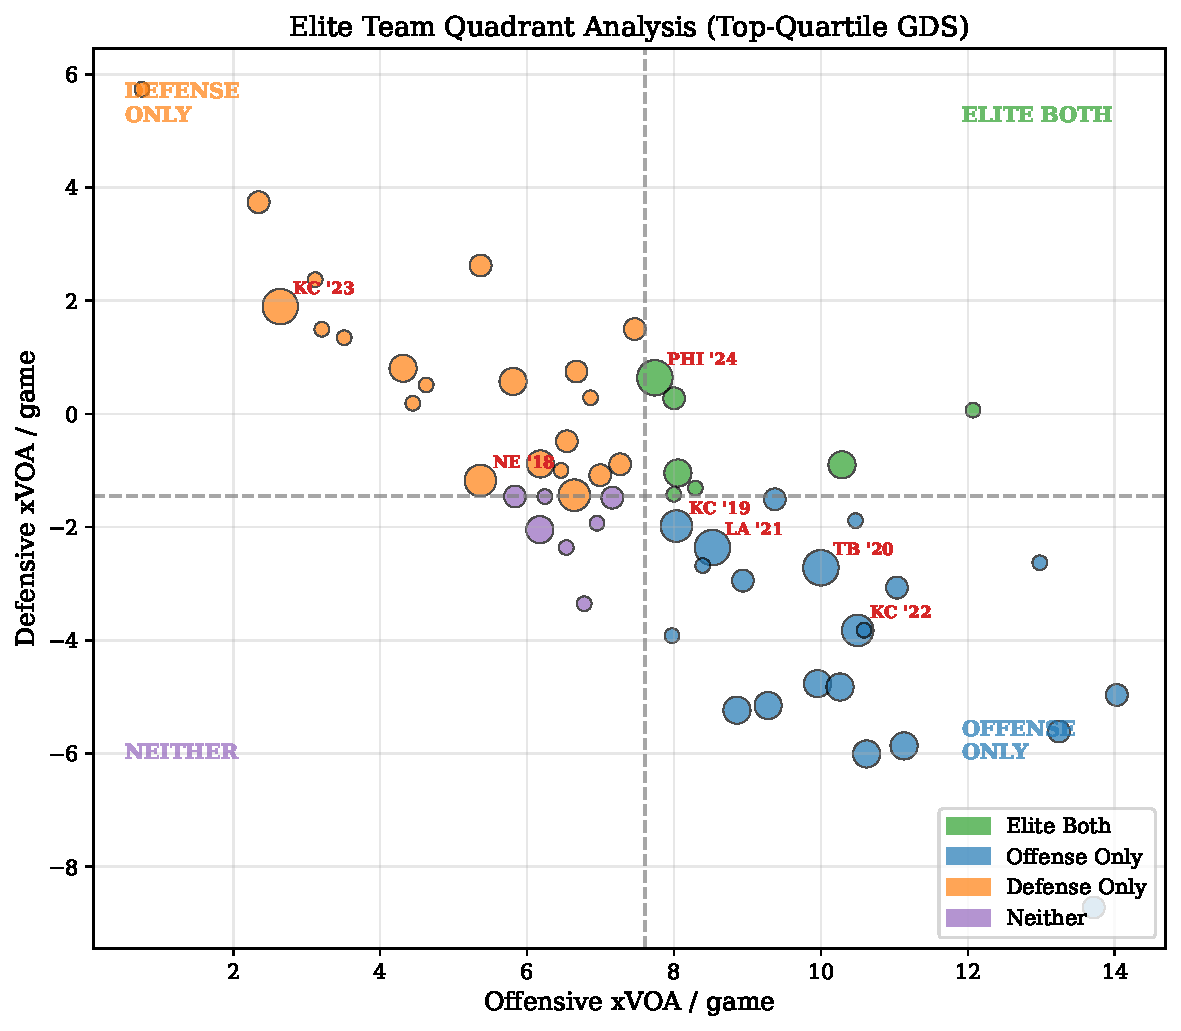
\includegraphics[width=0.8\textwidth]{../../thesis/figures/fig10_quadrant_diagram.pdf}
  \caption{Elite team quadrant analysis. Each point is a top-quartile \gds{}
           team-season, positioned by offensive (x-axis) and defensive (y-axis)
           \xvoa{}/game. Dashed lines indicate within-elite medians. Super Bowl
           winners are annotated.}
  \label{fig:quadrant}
\end{figure}

The most striking finding is the \textit{Offense Only} quadrant's dominance of championship production. Across 21 elite team-seasons with above-median offensive \xvoa{} but below-median defensive \xvoa{}, four won the Super Bowl (19.0\% rate). These teams -- Kansas City 2019, Tampa Bay 2020, the Los Angeles Rams 2021, and Kansas City 2022 -- achieved championships with below-median defensive contributions within the elite tier, carried by dominant offenses. The mean playoff wins (1.52) and conference championship rate (47.6\%) are the highest among all four quadrants.

The \textit{Defense Only} quadrant, by contrast, produced two Super Bowl winners (New England 2018, Kansas City 2023) for a 9.5\% rate -- exactly half the \textit{Offense Only} rate. Mean playoff wins in \textit{Defense Only} (1.10) trail \textit{Offense Only} (1.52) by 0.42 wins, and conference championship rates follow the same pattern (28.6\% vs.\ 47.6\%). The \textit{Offense Only} pathway produced more championships (4) than all other quadrants combined (3).

The \textit{Elite Both} quadrant ($n = 7$) records a 14.3\% Super Bowl win rate and 42.9\% conference championship rate, driven by Philadelphia 2024. While the per-team probability is high, the smaller sample limits total championship production. The \textit{Neither} quadrant ($n = 7$) produced zero Super Bowl wins and the lowest mean playoff wins (0.57), confirming that elite total \gds{} alone -- without strong performance in at least one major phase -- does not translate to championship contention.

The practical implication: among elite teams, having above-median offense is the strongest predictor of championship success regardless of defensive quality, and the \textit{Offense Only} pathway is more productive than the \textit{Defense Only} pathway by a factor of two in championship rate.

\subsection{Robustness and Sensitivity}
\label{sec:robustness}

\subsubsection{Opponent-Strength Control}

The OLS model is re-estimated with the leave-one-out opponent-strength variable included as a covariate:
\begin{align*}
  R^2 &= 0.255, \\
  \hat{\beta}_1(\text{off\_xvoa/g}) &= 0.099 \quad (p < 0.0001), \\
  \hat{\beta}_2(\text{def\_xvoa/g}) &= 0.065 \quad (p = 0.0001), \\
  \hat{\beta}_3(\text{opp\_avg\_gds}) &= -0.001 \quad (p = 0.985).
\end{align*}
The opponent-strength coefficient is effectively zero ($-0.001$) and entirely non-significant ($p = 0.985$), with no material change to either the offensive or defensive coefficient or to model $R^2$. The opponent-strength variable ranges from $-1.95$ to $+1.89$ across the sample, indicating meaningful variation in schedule difficulty -- yet this variation bears no relationship to playoff advancement after controlling for team quality. This null result directly addresses the schedule-strength confound: the offensive advantage is not an artifact of offense-dominant teams systematically facing weaker schedules. The offensive \xvoa{} coefficient remains unchanged at $0.099$ ($p < 0.0001$), confirming that the offensive advantage represents genuine execution quality independent of opposition strength.

\subsubsection{Field-Position Mediation}

A mediation analysis tests whether defensive quality inflates offensive \xvoa{} through a field-position channel. The correlation between defensive \xvoa{}/game and the team's average starting field position advantage is $r = -0.193$ ($p = 0.0037$), confirming that better defenses do generate modestly superior starting positions for their offenses -- the mediating pathway exists but is weak. The total correlation between offensive \xvoa{}/game and playoff wins is $r = 0.443$; the partial correlation controlling for average starting field position advantage is $r_{\mathrm{partial}} = 0.402$. The mediation percentage:
\[
  \text{Mediation} = \frac{0.443 - 0.402}{0.443} = 9.2\%.
\]
Only 9.2\% of the association between offensive \xvoa{} and winning is attributable to defense-generated field position. The remaining 90.8\% operates independently of any defensive contribution. This finding directly addresses the concern that offensive \xvoa{} is ``really'' measuring downstream effects of defensive quality: the data show that it is overwhelmingly measuring independent offensive execution. Good defenses do generate modestly better starting positions, but this indirect pathway accounts for less than one-tenth of the total offensive contribution to winning.

\subsubsection{Time-Window Sensitivity}

\Cref{tab:sensitivity-time} reports the offensive-to-defensive $R^2$ ratio across five overlapping time windows.

\begin{table}[htbp]
  \centering
  \caption{Sensitivity of the offensive-to-defensive $R^2$ ratio to time
           window selection. The ratio remains above 2:1 across all windows,
           confirming structural stability.}
  \label{tab:sensitivity-time}
  \begin{tabular}{lcc}
    \toprule
    \textbf{Window} & \textbf{$R^2$ Ratio (Off:Def)} & \textbf{$n$ (team-seasons)} \\
    \midrule
    2018--2024 (full)   & 3.3 : 1 & 224 \\
    2018--2022          & 3.0 : 1 & 160 \\
    2019--2024          & 3.0 : 1 & 192 \\
    2020--2024          & 4.0 : 1 & 160 \\
    2018--2021          & 2.5 : 1 & 128 \\
    \bottomrule
  \end{tabular}
\end{table}

Across all windows, offensive quality explains between 2.5 and 4.0 times as much win-rate variance as defensive quality. No window produces a ratio below 2:1, confirming that the offensive advantage is structurally stable and not driven by a single anomalous season. The range of 2.5 to 4.0 indicates that the 3.3:1 full-sample ratio is representative rather than extreme.

\subsubsection{Threshold Sensitivity}

\begin{table}[htbp]
  \centering
  \caption{Sensitivity of defense-dominant playoff performance to archetype
           threshold. Defense-dominant teams record zero mean playoff wins
           regardless of classification boundary.}
  \label{tab:sensitivity-threshold}
  \begin{tabular}{lcc}
    \toprule
    \textbf{Threshold} & \textbf{$n$ (Def-Dominant)} & \textbf{Mean PW} \\
    \midrule
    $\pm 0.20$ & 38  & 0.000 \\
    $\pm 0.25$ & 34  & 0.000 \\
    $\pm 0.30$ & 29  & 0.000 \\
    $\pm 0.35$ & 26  & 0.000 \\
    $\pm 0.40$ & 24  & 0.000 \\
    \bottomrule
  \end{tabular}
\end{table}

Defense-dominant teams record zero mean playoff wins across all threshold specifications from $\pm 0.20$ to $\pm 0.40$. Whether the archetype definition is broadened (including teams with moderate defensive tilts, $n = 38$) or narrowed (requiring extreme defensive dominance, $n = 24$), no specification produces positive playoff success for defense-dominant teams. This result is robust to substantial variation in the classification boundary.

\subsubsection{Single-Team Exclusion}

Kansas City 2023 has the lowest offense share among Super Bowl champions ($+0.581$) and is the most frequently cited counter-example. Excluding this team-season from the analysis produces an $R^2$ ratio of 3.3:1 (unchanged) and a Spearman correlation between offense share and playoff wins of $\rho = 0.263$ ($p = 0.011$). No primary finding is dependent on the inclusion or exclusion of this observation.

\subsubsection{Era Comparison}

\begin{table}[htbp]
  \centering
  \caption{Era comparison of correlations. Spearman: offense share vs.\
           playoff wins (playoff teams only). Pearson: \xvoa{} components
           vs.\ win percentage (all team-seasons).}
  \label{tab:era}
  \begin{tabular}{lrrr}
    \toprule
    \textbf{Measure} & \textbf{2018--2020}
      & \textbf{2021--2024} & \textbf{$\Delta$} \\
    \midrule
    Spearman $\rho$ (share vs PW)      & $0.309$ & $0.221$ & $-0.088$ \\
    Sample ($n$, playoff teams)        & 38      & 56      & \\[4pt]
    Pearson $r$ (off \xvoa{} vs Win\%) & $0.621$ & $0.739$ & $+0.118$ \\
    Pearson $r$ (def \xvoa{} vs Win\%) & $0.397$ & $0.364$ & $-0.033$ \\
    \bottomrule
  \end{tabular}
\end{table}

The Spearman correlation between offense share and playoff wins remains positive in both eras (0.309 in 2018--2020, 0.221 in 2021--2024), confirming that offense share predicts playoff advancement regardless of the time period. The apparent attenuation in the 2021--2024 era may be partially influenced by the expanded playoff field (14 teams vs.\ 12), which admits more marginal qualifiers and compresses offense-share variance among playoff teams.

The Pearson correlations reveal a modest strengthening of the offensive channel in the 2021--2024 era (0.621 to 0.739) alongside a slight weakening of the defensive channel (0.397 to 0.364). This directional pattern is consistent with the hypothesis that the post-2021 rule environment has slightly amplified the predictive value of offensive execution, though the magnitudes are small and era subsamples are insufficient for formal inference.

The key finding is directional consistency: whether examined in 2018--2020 or 2021--2024, the direction of evidence is the same -- offense is the stronger predictor. No era shows a reversal in which defensive dominance emerges as the primary pathway.

\subsection{Hypothesis Verdict}

All three hypotheses are rejected across every analytical method employed. No defense-dominant team reached a conference championship game. Across 224 team-seasons and 94 playoff appearances, the weight of evidence consistently and strongly favors offense. The convergence across correlational, variance-explained, effect-size, regression, and descriptive analyses provides the strongest available evidence against the defensive championship hypothesis in the 2018--2024 NFL. The data are inconsistent with all three formulations of the ``defense wins championships'' claim in both direction and magnitude.

% ============================================================
% 5. DISCUSSION
% ============================================================
\section{Discussion}
\label{sec:discussion}

\subsection{Rejecting the Defensive Hypothesis}
\label{sec:rejecting}

The central empirical question -- whether defensive dominance is the primary pathway to championship success in the modern NFL -- receives an unambiguous answer. All three pre-specified hypotheses are rejected, and the rejection is not marginal or dependent on a particular procedure. It is consistent across all five statistical tests, both descriptive partitioning strategies, and both era subsamples.

The convergence across methods is what distinguishes this finding from prior work. Each procedure -- Spearman correlation, Pearson $R^2$ decomposition, Cohen's $d$, logistic regression, OLS -- independently favors offense by a substantial margin. No procedure produces evidence in the defensive direction, and no robustness check attenuates the result.

The most striking finding is the complete absence of defense-dominant success: among 29 defense-dominant team-seasons, zero won any playoff games, zero reached a conference championship, and zero appeared in a Super Bowl. This null result stands against 94 total playoff team-seasons across seven seasons -- a sample large enough that complete absence cannot reasonably be attributed to chance alone. The seven offense-dominant champions, with shares ranging from $+0.581$ to $+0.923$, represent the categorical pattern: within this seven-season window, no team won a championship without an offense-dominant profile.

\subsection{The Competent Defense Threshold}
\label{sec:threshold}

The rejection of the defensive hypothesis should not be misinterpreted as a claim that defense is irrelevant to winning championships. The data suggest a more refined structural interpretation: offensive quality is the primary engine of playoff qualification and advancement, while competent defense serves as a necessary -- but not sufficient -- condition at the championship margin. The distinction between being the \emph{driver} of success and being a \emph{filter} for the final stage is crucial. Offense determines which teams reach the deep postseason; among teams that arrive there, defensive adequacy helps determine which survives elimination rounds.

Kansas City's 2023 Super Bowl victory illustrates this ``balanced elite'' archetype and provides the strongest test case for the defensive narrative. Often characterized in popular discourse as a ``defense-led'' championship, the \gds{} decomposition reveals a more nuanced picture: the 2023 Chiefs had positive offensive \xvoa{} ($+2.641$/game) alongside positive defensive contribution ($+1.896$/game), yielding an offense share of $+0.581$ -- the lowest among champions but still firmly offense-dominant. The popular narrative that Kansas City won ``because of their defense'' is not supported by the expected-point framework: the offense generated more absolute value than the defense. What distinguishes this championship is that defensive quality contributed more \emph{relative to other champions}, not that it was the primary engine.

The concept of a ``competent defense threshold'' emerges naturally from the data. Five of seven champions recorded \emph{negative} defensive \xvoa{}/game -- their defenses performed below league-average expectations at the drive level. Kansas City 2022 won the Super Bowl with defensive \xvoa{} of $-3.826$/game, substantially below average. The threshold for championship viability appears remarkably low: teams can win the Super Bowl with below-average defense provided their offensive surplus is sufficiently large. A team with elite offense and below-average defense (Kansas City 2022) can win the championship. A team with elite defense and below-average offense has not done so in seven seasons of data. The threshold is asymmetric: the minimum offensive requirement for championship contention is substantially higher than the minimum defensive requirement.

The quadrant analysis reinforces this interpretation. Among elite teams, \textit{Offense Only} produced four champions (19.0\%) versus two for \textit{Defense Only} (9.5\%), despite identical sample sizes. The championship rate for teams with above-median offense regardless of defensive quality is double that of teams with above-median defense regardless of offensive quality. Defense matters, but it matters less.

\subsection{Structural Explanations}
\label{sec:structural}

Three mechanisms explain why offensive quality is the stronger differentiator in the modern NFL, providing structural grounding for what might otherwise appear as a mere statistical regularity.

First, offensive production exhibits higher between-team variance than defensive production. The standard deviation of offensive \xvoa{}/game across team-seasons exceeds that of defensive \xvoa{}/game. Higher variance in a predictor variable mechanically produces stronger correlations with outcomes because the variable provides more discriminating information between observations. The gap between the best and worst offenses in the NFL is wider than the gap between the best and worst defenses, reflecting structural realities: offensive schemes are more diverse (from Shanahan-system run games to Air Raid passing attacks), quarterback quality varies more dramatically across rosters than any defensive position, and the passing game creates more opportunity for between-team separation than the constrained action space of defensive play.

Second, the post-2018 rule environment systematically amplifies offensive variance while compressing defensive impact. Increased enforcement of pass interference, expanded roughing-the-passer protections, and restrictions on defensive contact beyond five yards \citep{pereira2018roughing, barnwell2019passingrevolution} have expanded the ceiling for offensive execution while compressing the floor for defensive impact. Even the most elite defensive units in the modern game cannot prevent completions to the degree possible before 2018, because the rules constrain the tools available to them -- physical coverage, press techniques, aggressive pass-rush angles are all more heavily penalized. The era analysis provides directional support: the offensive Pearson coefficient strengthens from 0.621 (2018--2020) to 0.739 (2021--2024), while the defensive coefficient shows no corresponding increase (0.397 to 0.364).

Third, offense possesses a structural ceiling advantage rooted in the proactive-reactive asymmetry of football. The best offenses can score on nearly any opponent in any game; the best defenses cannot prevent all scoring against any opponent. Offense chooses the terms of engagement -- formation, personnel grouping, play-call, tempo, motion -- while defense reacts within the framework the offense establishes. This proactive-reactive asymmetry means that schematic innovation accrues disproportionately to the offensive side, where coordinators can design novel concepts (new motion patterns, formation shifts, RPO combinations) that defenses have not yet adapted to. Defensive innovation is constrained to adjustments within the opponent's chosen framework, a fundamentally more limited strategic space.

\subsection{Why the Myth Persists}
\label{sec:myth}

If the evidence so clearly favors offense, the persistence of the ``defense wins championships'' narrative requires explanation. Several cognitive and structural factors conspire to sustain the belief despite its empirical weakness.

The most powerful is availability bias combined with a denominator problem \citep{tversky1973availability}. The Super Bowls that dominate collective memory are disproportionately those with spectacular defensive performances: Seattle 2013 dismantling Peyton Manning's record-setting offense, Denver 2015 winning with an aging quarterback behind a dominant defense. These games are memorable precisely because they are \emph{unusual} -- a defense-dominant team winning the championship is a departure from the base rate, which makes it cognitively salient. The seven offense-dominant champions in this study's window do not generate comparable narrative drama; a team with the best offense winning is unremarkable, and unremarkable events do not anchor in memory. The ease with which defensive championship performances come to mind is mistaken for their frequency.

The denominator problem compounds this bias. Observers notice when a defense-dominant team wins a championship because the event is visible and celebrated. They do not notice the far more frequent occurrence of defense-dominant teams failing to reach the championship stage -- because absences are invisible. The data make this absence concrete: only six defense-dominant teams (offense share $< 0$) even made the playoffs across seven seasons, and none won more than a single game. These quiet exits receive no media attention, no retrospective analysis, and no cultural narrative. The myth persists partly because the denominator -- defense-dominant teams that failed -- is never examined.

Additionally, the narrative possesses a romantic appeal that transcends evidence. The David-versus-Goliath framing -- a tough, physical defensive team outmuscling a flashy offense -- resonates with cultural values of effort, grit, and determination. It suggests that talent and scheme can be overcome by intensity, a more satisfying story than the alternative: that the team with better players executing a better offensive scheme typically wins. Confirmation bias in real-time viewing reinforces this -- low-scoring games are attributed to ``defensive dominance'' rather than to the more prosaic explanation of offensive ineptitude on both sides.

\subsection{Strategic Implications}
\label{sec:strategic}

The salary cap's zero-sum structure means the 3.3:1 $R^2$ ratio carries direct resource allocation implications -- conditional on these associations at least partially reflecting causal mechanisms. If marginal offensive investment yields higher expected returns than marginal defensive investment, the traditional ``balance'' philosophy -- treating offense and defense as symmetric inputs with symmetric returns -- may be suboptimal. A team allocating asymmetrically toward offense is not ``unbalanced'' in any meaningful strategic sense; it is responding to the empirical evidence that offensive quality has nearly three times the predictive association with winning \citep{mulholland2019optimizing}.

This consideration challenges conventional front-office philosophy but must be bounded by the competent defense threshold. The recommendation to overweight offense does \emph{not} imply minimizing defense to zero. Catastrophic defensive failure -- the extreme lower tail of the distribution -- can override even positive offensive production. The strategic objective is ``offense-first, with defensive catastrophe avoided.'' The data show that moderately below-average defense (the range occupied by five of seven champions) is tolerable, but extreme defensive weakness is not. The optimal allocation is not ``all offense'' but ``offense-first with a defensive floor'' -- the difference between a reckless gamble and a disciplined capital allocation strategy informed by evidence.

All strategic implications carry an essential caveat: these are correlational findings, not causal demonstrations. The analysis documents patterns of association between team quality components and competitive outcomes. It does not prove that investing in offense \emph{causes} teams to win more. The strategic implications are therefore conditional: they follow if the observed associations at least partially reflect causal mechanisms, and they should be interpreted as directional hypotheses warranting further investigation rather than proven prescriptions. Organizations considering these implications should weigh them alongside domain expertise, contextual knowledge, and the inherent limitations of observational evidence.

\subsection{Limitations}
\label{sec:limitations}

Several limitations constrain the strength of these conclusions.

First, the seven-season window (2018--2024) limits generalizability to this specific rule era. The study window coincides with an NFL environment that explicitly favors offensive production through expanded protections and contact restrictions. Whether the offensive advantage documented here is a structural truth about football or a rule-era artifact cannot be determined from these data alone. Future rule changes rebalancing offense and defense could attenuate the observed advantage. A longitudinal extension spanning multiple regulatory eras (2002--2024 or longer) would be required to disentangle structural from rule-induced effects.

Second, the \gds{} framework measures raw execution quality without adjusting for opponent quality at the drive level. A defense achieving high \xvoa{} against below-average offenses is rated identically to one facing elite opponents. The season-level OLS control was null ($\hat{\beta}_3 = -0.001$, $p = 0.985$), providing empirical reassurance that schedule-strength confounding does not materially affect the archetype findings. Nevertheless, a principled drive-level opponent adjustment -- in which each drive's expected baseline accounts for the opposing unit's quality via iterative estimation -- would further strengthen internal validity.

Third, and most consequentially, the analysis documents statistical associations rather than causal relationships. The finding that offensive \xvoa{} covaries more strongly with winning demonstrates correlation, not that investing in offensive talent \emph{causes} teams to win more games. A specific concern is reverse causation through game state: teams that establish early leads shift to conservative play-calling, which may systematically affect their \xvoa{} profiles. The \xscore{} model partially mitigates this by conditioning on score differential (so expected values already account for game script), but this mitigation is incomplete. The strategic implications drawn in the previous section rest on the assumption that associations partially reflect causal mechanisms -- an inference rather than a demonstration.

Fourth, the logistic regression is substantially underpowered. With 7 Super Bowl events and 2 predictors, the events-per-variable ratio is 3.5, well below the standard recommendation of 10 \citep{peduzzi1996simulation, hosmer2013logistic}. Coefficient estimates carry substantial uncertainty, and the model has limited power to detect effects of moderate size. The primary evidential basis rests on the full-sample tests ($n = 94$ playoff team-seasons, $n = 224$ total), not the championship-specific logistic model alone.

Fifth, the era subsamples (38 and 56 playoff team-seasons) are insufficient for formal inference on temporal trends. The era comparison is explicitly exploratory. The per-era Spearman coefficients cannot be formally tested for significant difference, and the directional pattern (both positive) is more informative than any magnitude comparison given the low statistical power of within-era tests.

Sixth, elite quarterback quality is a potential confound. Elite quarterbacks simultaneously drive both offense share (through their direct contribution to offensive \xvoa{}) and playoff success (through leadership, clutch performance, and experience effects). The observed offensive advantage may therefore partially reflect the concentrated importance of the quarterback position rather than broader offensive investment. Disaggregating quarterback-driven value from scheme and supporting-cast value is beyond the scope of this analysis but represents a productive direction for future work with player-level \xvoa{} attribution.

% ============================================================
% 6. CONCLUSION
% ============================================================
\section{Conclusion}
\label{sec:conclusion}

Across 224 team-seasons, five statistical procedures, and a comprehensive suite of robustness checks, the evidence systematically contradicts the ``defense wins championships'' hypothesis in the modern NFL. Offense-dominant teams dramatically outperform defense-dominant teams in playoff advancement (Cohen's $d = 0.672$), offensive \xvoa{} explains 3.3 times more win-percentage variance than defensive \xvoa{} (46.4\% vs.\ 14.2\%), all seven Super Bowl champions were offense-dominant, and no defense-dominant team won more than one playoff game across 94 playoff team-seasons. These findings are robust to opponent-strength controls, field-position mediation, threshold and time-window sensitivity, and single-team exclusion.

This paper contributes the first multi-method test of the defensive hypothesis using a calibrated machine-learning team quality decomposition. It substantially extends \citet{robst2011defense} -- the only prior peer-reviewed examination -- with drive-level measurement that conditions on game state, a modern sample spanning the current rule era, five converging statistical procedures with pre-specified directional hypotheses, and full open-source reproducibility. The ``competent defense threshold'' framework provides a theoretical contribution beyond mere hypothesis rejection: offensive excellence drives championship contention while defensive adequacy serves as a necessary but insufficient secondary condition. Five of seven champions won with below-average defensive \xvoa{} -- the threshold for championship viability is remarkably low on the defensive side.

The practical takeaway for team construction under the salary cap is not ``all offense'' but recognition that the 3.3:1 variance ratio implies asymmetric marginal returns under a binding constraint. Teams should invest to maintain defensive adequacy while maximizing offensive ceiling, recognizing that the traditional ``balance'' philosophy treats asymmetric inputs as if they were symmetric -- a form of suboptimal allocation that the portfolio theory literature would recognize as leaving expected value on the table.

Several extensions would strengthen and broaden these conclusions. Longer time horizons extending to 2002 or earlier, with appropriate era controls, would test whether the offensive advantage is a modern phenomenon or a structural constant. A drive-level opponent adjustment via iterative strength-of-schedule corrections would address the remaining internal validity concern. Positional value decomposition -- separating offensive \xvoa{} into rushing and passing components -- would identify which specific offensive investments carry the highest marginal championship returns. Player-level \xvoa{} attribution would connect team-level findings to individual talent evaluation and draft strategy. Finally, salary-cap efficiency analysis relating \gds{} components to positional cap expenditure would directly quantify market inefficiencies and test whether the ``defense wins championships'' heuristic has measurably distorted the talent market in ways that analytically sophisticated organizations could exploit. For complete technical details, the full robustness analysis, and extended era-stratified results, see the companion thesis \citep{mecha2026xscore}.

The evidence does not merely fail to support ``defense wins championships'' -- it systematically contradicts it across every analytical method employed. The most widely cited strategic heuristic in professional football lacks empirical foundation in the modern game.

% ============================================================
% DATA AND CODE AVAILABILITY
% ============================================================
\section*{Data and Code Availability}

All play-by-play data are publicly available via the \texttt{nflfastR} package \citep{carl2021nflfastr}. The complete analytical codebase -- including archetype classification, statistical testing, and figure generation -- is available at \url{https://github.com/lasse5mecha/nfl-xscore-gds}.

% ============================================================
% CONFLICTS OF INTEREST
% ============================================================
\section*{Conflicts of Interest}

The author declares no conflicts of interest.

% ============================================================
% AI DISCLOSURE
% ============================================================
\section*{Statement on Use of Artificial Intelligence}

This paper was developed with the assistance of Claude (Anthropic), a large language model used as a coding and writing tool. All research design decisions, hypothesis operationalization, and interpretation of results are solely the author's intellectual contributions. AI-generated code was reviewed and validated by the author.

% ============================================================
% REFERENCES
% ============================================================
\printbibliography

\end{document}
